\chapter{Toolchain Backend}\label{chap:offline_tezos}
After parsing and transforming a list of assertions, the resulting ASTs are passed to the target-specific backend. For this thesis, the platform target is Tezos, with Michelson as the compilation target. The pipeline stages of the backend comprise the ones colourized in \figref{fig:pipeline_backend}. First, the generic ASTs are subjected to a semantic check, which rejects any assertions containing unsupported types, operations or other invalid expressions. Valid ASTs are then cast to a target specific AST type and passed to the type checker. In this stage, the assertions are linked to the respective parent entrypoints based on the parameter patterns and tags. Given the list of target specific ASTs and a linking, the compiler finally generates target code. Each stage is described in more detail in \secref{sec:backend_impl}.

As a preliminary for the compiler implementation, \secref{sec:ext_michelson} identifies necessary extensions to Michelson and Tezos' VM in order to facilitate the distributed assertion scheme. Although the extensions are formalized in this thesis, implementing the extension is part of the protocol amendment. Furthermore, the compiler needs to generate the target code according to an on-chain orchestration scheme between the assertion and parent contract. \secref{sec:orchestration} explores possible strategies for such a scheme, and discusses their strengths and weaknesses. Based on a resulting proposal for the orchestration, \secref{sec:cost_analysis_distributed} performs a cost analysis of the approach of distributed assertion checking and evaluates if, and under which conditions, it can solve the issue of scalability in blockchain applications.

As a foundation for the other sections, \secref{sec:tezos} provides important background on the Tezos blockchain, its built-in Smart Contract language Michelson and some relevant tools and projects within its ecosystem.

\section{Tezos}\label{sec:tezos}
The Tezos blockchain is presented in its whitepaper as a \enquote{generic and self-amending crypto-ledger} \cite{goodman_tezos_2014}. It uses a proof-of-stake consensus mechanism, which is not only used to agree on the current state of its ledger, but also allows its stakeholders to come to a consensus about changes in the economic protocol by participating in a voting process. The changes included in a protocol upgrade, called amendment, can influence i.a. which transactions are valid on the blockchain, the payment system or even the voting process itself. It does so without risking a fork of the blockchain. Everyone owning the cryptocurrency of Tezos, called Tez, is considered a stakeholder and can participate in the consensus mechanism. The whitepaper compares the self-amending protocol of Tezos to a game created by Philosopher Peter Suber called ``Nomic'', whose set of rules are subjected to a democratic voting system \cite{nomic}. Similar concepts can also be found in modern pop culture, such as the virtual sports league ``Blaseball'' \cite{blaseball}, which became popular during the COVID-19 pandemic.

In addition to user accounts associated with a public key, Tezos supports smart contracts, which are written in the built-in language Michelson. Tezos' transaction fee system is similar to that of Ethereum \cite{wood_ethereum_2021} - it is gas-instrumented and besides a base fee, every operation and byte of storage during contract execution has to be paid for by the user. However, Tezos imposes a hard cap on the amount of gas that can be consumed per operation (including internal transactions) \cite{tezos_docs}\cite{morley_repo}, whereas Ethereum limits the gas quota only in respect to blocks \cite{wood_ethereum_2021}.\\
Tezos is written in the multi-paradigm programming language OCaml. Compiling its source code yields five essential binaries: the  node, baker, endorser, accuser and client. The node is the entity connecting to the peer-to-peer network and keeping a copy of the chain. Bakers are responsible for producing new blocks, the endorsers for validating and signing new blocks and the accusers to call out bakers or endorsers which double-sign or -endorse. The client provides a command line interface to interact with nodes through remote procedure calls (RPC).

\subsection{Proof-of-stake in Tezos}
In Tezos, contracts which have staked a minimum amount of tokens, called a roll, can participate in the consensus mechanism. When participating, a contract has a chance to obtain the role of either a baker or an endorser. Contracts who don't own enough tokens, or infrastructure, to participate directly, can delegate their baking and endorsing rights to other contracts. The rights to bake or endorse are determined and assigned at the beginning of each cycle, which consists of a specified number of blocks. For baking, a random roll is selected for each block level and the rights are assigned to its owner. The block produced by that baker is signed by a fixed number of endorsers (32 as of protocol 007 Delphi), which also have been assigned endorsing rights for this block level by a random selection of rolls. Since participants can stake more than one roll, they may be assigned several endorsement slots at the same block level.

As an incentive for active participation in the consensus algorithm, delegates (and also delegators) receive rewards in form of tokens. However, if accusers detect double-baking or -endorsement, the delegate is penalized by burning (i.e., destroying) their security deposit.

\subsection{Michelson}
Michelson is a lower-level, stack-based language with strict type-checking. It supports primitive data types, like integers or strings, as well as high-level data structures, such as list, maps and sum types. The type system reduces the occurrence of runtime errors and ensures that only well-typed contracts are originated on the blockchain.

The concrete syntax of Michelson is called Micheline. A program is represented as Micheline nodes, which can be one of the following constructs:
\begin{itemize}
\item A constant of type integer (in decimal notation)
\item A constant of type string
\item A byte sequence in hexadecimal notation
\item An application of a language primitive to a sequence of nodes
\item A sequence of nodes
\end{itemize}
For documentation, readability and additional type constraints, Michelson and Micheline also offer three types of annotations - type, variable and field or constructor annotations, which are labelled with a unique special character in Micheline. The toplevel structure of a Smart Contract consists of a sequence of the three primitives \texttt{parameter, storage} and \texttt{code}. They declare the type of the input parameter, the storage type and the script, which is interpreted when the contract is invoked. The full grammar of Micheline and Michelson can be found in the Tezos developer resources \cite{tezos_docs}.

\subsubsection{Entrypoints}
Unlike Ethereum's contract language Solidity, Michelson doesn't have a concept of named functions with a dedicated parameter type. Instead of named functions, Michelson contracts models separate entrypoints by taking a sum type as an input parameter. The type constructors can optionally be tagged a field annotation, which can be considered an entrypoint name. The sum type is built by nesting the \texttt{or} type, which has the constructors \texttt{left} and \texttt{right}.

As an example, the contract in \lstref{lst:entrypoints} has two entrypoints --- entrypoint \texttt{A}, which expects an integer wrapped in the \texttt{left} constructor, e.g. \texttt{left 1}, and entrypoint \texttt{B}, which expects a string wrapped in the \texttt{right} constructor, e.g. \texttt{right "hello world"}.
\begin{lstlisting}[language=Michelson, numbers=none, caption=Michelson contract with two entrypoints, label=lst:entrypoints]
parameter (or (int %A) (string %B));
storage unit;
code {
  ...
  IF_LEFT { ... (* entrypoint A *)}
          { ... (* entrypoint B *)}
}
\end{lstlisting}
By adding the constructor annotations \texttt{A} and \texttt{B}, the entrypoints can be invoked explicitly. The passed parameter value is then wrapped automatically into the respective constructor. Furthermore, it's possible to declare a \texttt{default} entrypoint, which is invoked when no explicit tag is specified in the transaction. By default, the default entrypoint is assigned to the root of the parameter type.

\subsubsection{Internal operations}
Smart Contracts are able to invoke other Smart Contracts by emitting internal operations. The return type of Michelson programs is a tuple of a list of internal operations and the updated storage. After a contract completes, the operations in the returned list are run in sequence. Since internal operations may in turn also emit internal operations, the interpreter puts all emitted operations into a queue, which is processed in order. As an example, \figref{fig:internal_ops} shows an execution order of two external transactions and their internal operations in sequence.
\begin{figure}[h]
\centering
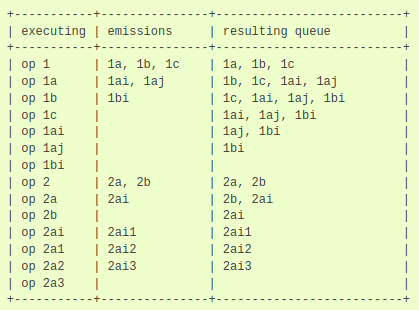
\includegraphics[width=0.5\linewidth]{figures/5-offline_tezos/internal_ops}
\captionsource{Execution order of two external operations and their internal operations}{\cite{tezos_docs}}
\label{fig:internal_ops}
\end{figure}

Both external and internal operations can fail, if the source contract does not have enough balance to spend the specified amount, a gas limit was reached, or if a program fails due to reaching a \texttt{FAILWITH} instruction. If a failure occurs, the whole sequence fails and all changes up to the point of failure are reverted.

\subsection{Gas model}
Tezos stores and transmits data as byte sequences --- in order to obtain a typed representation of their value for interpretation, a byte sequence is first deserialised into Micheline and subsequently parsed into a typed AST. Conversely, before transmitting or storing something on the blockchain, the typed representation is first unparsed into Micheline and then serialised. Since these working steps also entail computational effort, they consume gas and thus account for some of the transaction fees. The gas consumption of an operation (e.g., a transaction or a contract origination) is thus composed of the following positions \cite{morley_gasmodel}\cite{tezos_repo} on top of a base gas fee:
\begin{enumerate}
\item \textbf{Reading costs} --- apply for reading the contract code and storage from the blockchain and, on top of a base cost, depend on the amount of bytes read
\item \textbf{Deserialization costs} --- depend on the Micheline expression and the size of the byte sequence
\item \textbf{Parsing costs} --- are composed of three types of costs:
	\begin{itemize}
	\item type parsing --- apply when a Micheline node is converted into a valid type
	\item data parsing --- apply when a node is converted into the value of a known type and depends on the size of the value
	\item code parsing --- apply when the instructions of a program are type checked and depends on the number and types of instructions. Some instructions are expensive, such as \texttt{IF} (both branches need to be checked and compared) or \texttt{CREATE\_CONTRACT} (requires type check of invoked contract)
	\end{itemize}
\item \textbf{Type comparison costs} --- apply when types are checked for equality (e.g. when type checking the branches of the \texttt{IF} instruction) or during contract interpretation
\item \textbf{Interpretation costs} --- apply for each interpreted instruction and depend on their complexity.
\item \textbf{Unparsing costs} --- apply when converting typed data to untyped Micheline nodes and depend on the data type and size
\item \textbf{Serialization costs} --- apply when serializing Micheline nodes to byte sequences and depend on the expression and its size
\item \textbf{Writing costs} --- apply when writing to the internal database and depend on the amount of bytes. A base fee applies for each additional byte of storage.
\end{enumerate}
If a transaction emits internal operations, their gas consumption is computed in the same way and are added to the total gas consumption of the external operation.

\subsection{Developer tools in the Tezos ecosystem}
This section describes some tools and projects within Tezos' ecosystem, which are relevant to the development of the toolchain or the protocol amendment.

\subsubsection{Tezos Libraries}
Tezos' executables and libraries are available on OCaml's package manager \texttt{opam} \cite{tezos_opam}. The protocol libraries of every version are released separately, thus any projects can be built on the protocol of choice. Relevant libraries included in the backend of the toolchain are, i.a, the Micheline library containing the internal abstract syntax tree (AST) and parser of the Michelson language, the protocol libraries providing functions to type check code or data, and client libraries to retrieve any needed information from the node or blockchain via wrapped RPCs.

\subsubsection{Testing tools}
Before a new protocol is proposed to the Tezos network, it has to be thoroughly tested with system, integration and regression tests. This requires a sandboxed network to simulate the real peer-to-peer network. Tezos' development environment provides the two testing frameworks Flextesa (Flexible network sandboxes)\cite{tezos_docs} and its successor Tezt \cite{tezos_docs}. They allow to configure and run a small, fully functional sandboxed test network including nodes, bakers, endorsers and accusers. Besides testing new protocols, they can also be used to interactively test Smart Contracts.

\subsubsection{High-level languages}
Michelson is a compilation target for various high-level languages that provide a more user-friendly and intuitive way of writing Smart Contracts. Additionally, some of them come with development environments, testing or verification tools. The following list introduces three prominent languages compiling to Michelson:
\begin{description}
\item[\textbf{Liquidity}] \cite{liquidity} is a language with an OCaml-like syntax, which allows using local variables instead of stack manipulations. Its module system can be used to write reusable contract code or libraries. Besides an optimizing compiler, the project also includes a decompiler to compile Michelson programs to Liquidity source code.
\item[\textbf{SmartPy}] \cite{smartpy} is a language available through a Python library and lets developers write contracts and tests using Python syntax and structures (such as classes). Its developer suite includes, i.a., a compiler, a simulation engine for testing contracts and an online editor.
\item [\textbf{Ligo}] \cite{ligo} offers multiple syntax flavours close to Pascal, OCaml or Reason. Besides compilation, the toolchain allows to invoke or evaluate the generated code locally. The project provides Ligo as OCaml packages, which can be integrated into other projects.
\end{description}

\section{Extensions to Michelson}\label{sec:ext_michelson}
For the assertion code to be executable by the VM of Tezos, Michelson and the VM have to be extended with new instructions. This includes an instruction to generate a random value of some primitive data type non-deterministically. The formalization and possible implementation of such an instruction is described in \secref{sec:random}. Aside from this, many useful use-cases involve checking random elements of lists, and possibly strings or bytes. For convenience, it is worth considering adding indexing operations for some data types to the VM. This is discussed in more detail in \secref{sec:nth}.

As a foundation for the formalization of these new instructions, \secref{sec:michelson_semantics} gives a brief introduction to the Michelson interpreter and type system first.  

\subsection{Language semantics and type system}\label{sec:michelson_semantics}
The way Michelson is interpreted is purely functional; the interpreter takes the current stack and an operation and builds a return stack from the initial one, without causing any side effects. The definition of the recursive interpreter is given in the form of a list of rules, comprising of all possible inputs (i.e., program and stack types) and the respective output stack type of the computation. Each rule is of the following form: 
\begin{lstlisting}[caption=Selection rules in the Michelson interpreter \cite{tezos_docs}, language=, numbers=none, label=lst:rules]
> (syntax pattern) / (initial stack pattern)  =>  (result stack pattern)
    iff (conditions)
    where (recursions)
    and (more recursions)
\end{lstlisting}
For each valid program and initial stack, exactly one rule matches. Following the keyword \texttt{iff}, the rule can add extra conditions over values on the stack. If the result depends on the results of other program interpretations, such as conditionals or function calls, the rule can contain \texttt{where} or \texttt{and} clauses. These clauses represent a recursive interpretation of an intermediate program. The rule thus only applies, if the interpretation of the intermediate result matches the expected pattern.

The type system of Michelson consists of typing rules for each syntax construct, restricting the valid input stacks. The typing rules use the meta variables \texttt{'a} for type, and \texttt{'A} for stack type variables. Using these meta variables, the rules express consistency within the program. The typing rules are given in the form shown in \lstref{lst:type_rules}, where premises are additional typing requirements over values on the stack:
\begin{lstlisting}[caption=Form of typing rules in Michelson's specification \cite{tezos_docs}, language=, numbers=none, label=lst:type_rules]
(syntax pattern)
:: (type of stack before) -> (type of stack after) [rule-name]
   iff (premises)
\end{lstlisting}
The Tezos developer resources \cite{tezos_docs} provide a comprehensive list of type notations, syntax and stack patterns.

Since the Michelson language and interpreter are implemented in the protocol-specific libraries of Tezos, adding new instructions require a protocol update. This entails adding the new instruction to the list of tokens, adding one or several selection rules to the interpreter and typing rules to the type checker \cite{tezos_repo}. Furthermore, the protocol must specify the gas cost of its computation. Previous extensions to the Michelson language, such as the addition of the instruction ``\texttt{DIG n}'' in protocol 005 Babylon \cite{tezos_michelson_ext}, can be used as a guideline for the extension. The gas cost specification of existing instructions \cite{tezos_repo_gas} should be used as an orientation in specifying the costs of new instructions.

\subsection{random}\label{sec:random}
Since Smart Contracts generally need to be deterministic, s.t. the network can reach a consensus about the state of the ledger \cite{chatterjee_probabilistic_2019}, the prevalent workarounds for generating pseudo-random numbers cannot be used to implement the random generators in assertion contracts. The scheme explicitly requires as many validators as possible to check distinct elements in the search space. Common schemes for obtaining random values, like oracles or using block attributes as seeds \cite{chatterjee_probabilistic_2019}, would provide the same values for all validators. Thus, the VM should provide an instruction to generate a ``real'' random value for assertion checking only. The instruction should not be available in the normal execution mode, in order to preserve the deterministic behaviour of normal Smart Contracts.

\lstref{lst:rand_type} specifies the typing and selection rule of a new instruction \texttt{random} for integers (such an instruction can also be provided for other data types, such as \texttt{nat}, \texttt{string} or \texttt{mutez}). It consumes an offset and a positive range from the stack and pushes a randomly generated integer to the top. The typing rule (line 1) specifies, that the offset should be of type \texttt{integer}, and the range of type \texttt{nat}.
\lstset{upquote=true}
\begin{lstlisting}[caption=Typing and selection rules of the integer \texttt{random} instruction, language=, showlines=true, label=lst:rand_type]
:: int : nat: 'A -> int : 'A
> RANDOM / offset : range : S  => int : S
\end{lstlisting}

Within the Michelson interpreter, the selection of rules is implemented as a huge match case \cite{tezos_repo}. If the rule for \texttt{random} applies, the instruction could be computed in OCaml as indicated in \lstref{lst:rand_impl}.
\begin{lstlisting}[caption=Simplified evaluation of \texttt{random} in the Michelson interpreter, language=, label=lst:rand_impl]
match (instruction, stack) with
...
| (Random (offset, (range, rest))) ->
   Random.self_init;
   let rand_int = offset + Random.int(range) in
   return (rand_int, rest)  (* resulting stack *)
\end{lstlisting}

\subsection{nth}\label{sec:nth}
Michelson currently does not provide any predefined indexed access operators for data types like lists, strings or bytes. Accessing a random element of a sequence can, of course, be implemented using low-level instructions. However, because such operations are used frequently in many of the given use-cases, adding it as a predefined primitive for some data types might be justifiable. This reduces the required code to express the indexing, and thus not only improves the readability of the contract code, but also lowers the costs of the contract origination and execution.

\lstref{lst:nth_type} specifies the typing and selection rules of an instruction \texttt{nth} to access the $n^{th}$ element of a list. It consumes a list with elements of type \texttt{'a}, and an index of type \texttt{nat} from the top of the stack. After the computation, on top of the resulting stack is an optional value of the element type \texttt{'a}. A selection rule (line 2 and 3) is given for each of the two possible result stack patterns.
\begin{lstlisting}[caption=Selection and type rule of the list \texttt{nth} instruction, language=, label=lst:nth_type]
:: (list 'a) : nat : 'A -> option 'a : 'A
> NTH / l : index : S  =>  Some 'a: S
     iff index is within bounds
> NTH / l : index : S  =>  None 'a: S
     iff index is out of bounds
\end{lstlisting}

Within the VM, Michelson lists are represented with OCaml's list type --- the computation of \texttt{nth} thus simply calls the \texttt{nth} function of the List module, as indicated in \lstref{lst:nth_impl}.
\begin{lstlisting}[caption=Simplified evaluation of \texttt{nth} in the Michelson interpreter, language=, label=lst:nth_impl]
match (instruction, stack) with
...
| (Nth ({elements = []; _}, (_, rest))) ->
  return ((None, rest)
| (Nth ({elements = es; length}, (index, rest))) ->
  let l_length = of_int length in
  if index <= l_length
    then return (Some (List.nth es index), rest)
    else return (None, rest)
\end{lstlisting}
\lstset{upquote=false}

As stated above, the indexing operation can also be translated to a sequence of already existing instructions. Michelson features instructions to execute a loop or iterate over a list, which can be used for such an implementation. An exemplary implementation of the operation \texttt{nth} for lists in the high-level language Liquidity is given by \lstref{lst:nth_liq} in appendix \ref{apx:nth}. The appendix also contains the corresponding Michelson code after compiling the source with the Liquidity compiler (\lstref{lst:nth_tz}).

\section{Orchestration of contract and assertions}\label{sec:orchestration}
So far, the assertion and parent contract have been considered separately. However, they have to be orchestrated on-chain, such that the assertion code is either invoked automatically before the parent code is executed, or the assertion code can be invoked directly by the validators. Furthermore, the orchestration should include a mechanism to determine and trigger the required number of test runs per validator. Depending on the orchestration strategy, the compiler then assembles the assertion and parent code into one or several Smart Contracts.

This section describes two possible approaches for an orchestration --- a monolithic and a modular approach. It also discusses, which of the given architecture is chosen for the implementation of distributed assertion checking, and why.

\subsection{Monolithic orchestration}
In the monolithic approach, the assertion an parent code are merged into a single Smart Contract. This tightly couples and unites the code in one self-contained unit. The assertion code can be merged into the parent contract in two different ways. As shown in \figref{fig:mono_eps}, the assertions can be appended to the original contract as separate entrypoints. Alternatively, the assertion code can by prepended to the code of the respective entrypoint and thus become an integral part of the program (as shown in \figref{fig:mono_insert}).
\begin{figure}[!htb]
\subfloat[Appending assertions as separate entrypoints\label{fig:mono_eps}]{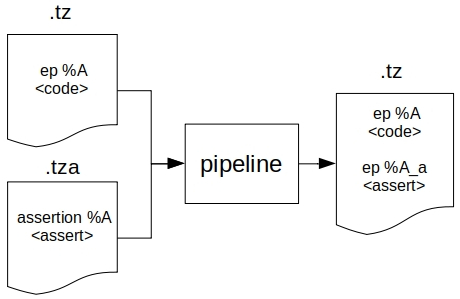
\includegraphics[width=0.5\textwidth]{figures/5-offline_tezos/pipeline_output_mono_ep_basic.jpg}}
\quad
\subfloat[Inserting the assertion code into the original entrypoint\label{fig:mono_insert}]{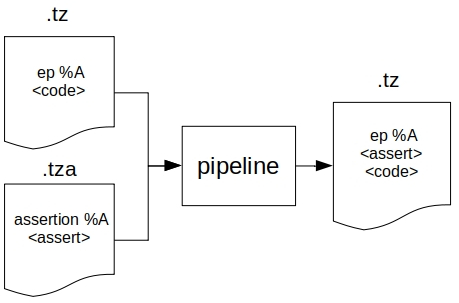
\includegraphics[width=0.5\textwidth]{figures/5-offline_tezos/pipeline_output_mono_basic.jpg}}
\caption{Approaches for the assembly of a monolithic contract}
\label{fig:monolithic_orchestration_basic}
\end{figure}

In variation (b), the link between the parent code and the respective assertion code is already established --- the assertion is executed automatically when invoking the entrypoint. Variation (a), on the other hand, still has to establish a link between the parent and the assertion entrypoint. It should be apparent, which of the entrypoints contains the original, and which one its respective assertion code. This can be solved by using fixed tag patterns for assertion entrypoints, which can be derived from the original entrypoint tag. \figref{fig:mono_eps} proposes the tag suffix ``\texttt{\_a}''. When an external transaction invokes such a monolithic contract, the bakers thus execute the contract normally. After completion, the baker then requests the validators to invoke the assertion separately. External transactions, of course, should only invoke the original entrypoints.

Both variations, however, do not yet provide any means to trigger several test runs per validator. Since only the contract itself knows how to calculate the required number of test runs $t$ (as per the range(s) of the random generator(s)), it cannot be passed to the validators as a parameter to the validation request. Instead, the contract itself needs to contain a controller to handle this. Similar to the assertion code, such a controller can be integrated into the parent entrypoint, or implemented as another separate entrypoint, as shown in \figref{fig:monolithic_orchestration}. Instead of invoking the assertion entrypoint (\texttt{A\_a}), the validators would then invoke the manager entrypoint (\texttt{A\_c}). This entryoint then determines $t$ and invokes the assertion entrypoint (\texttt{A\_a}) $t$ times as an internal operation. 
\begin{figure}[h]
\centering
  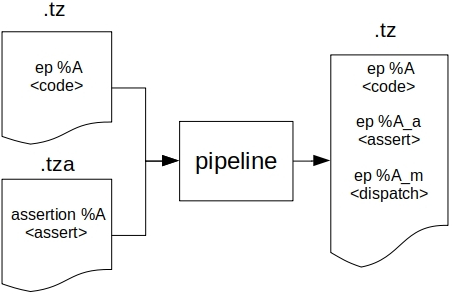
\includegraphics[width=0.5\textwidth]{figures/5-offline_tezos/pipeline_output_mono_ep.jpg}
	\caption{Monolithic assembly with separate entrypoints for manager and assertion}
	\label{fig:monolithic_orchestration}
\end{figure}

As a hybrid solution between a monolithic and a modular approach, the controller can be implemented as a separate Smart Contract, which operates as a proxy. This contract is invoked in pace of the monolithic contract, which in turn invokes the original or assertion entrypoints as internal operations. The implementation of the modular part can be adopted from \secref{sec:modular}.

If a developer did not specify an assertion for all entrypoints of the parent contract, invoking their non-existing controller entrypoints would cause a transaction failure. To avoid this and thus increase the robustness, the compiler should generate dummy controllers for empty assertions. If the monolithic contract is assembled according to \figref{fig:mono_eps}, the dummy controller simply returns unit (i.e, an empty list of internal operations and the unchanged storage). For the variation given in \figref{fig:mono_insert}, the controller invokes the original entrypoint exactly once.

\lstref{lst:mono_liq} implements a monolithic contract in the high-level language Liquidity. The contract contains the two parent entrypoints \texttt{A} (line 3) and \texttt{B} (line 21), and provides an assertion entrypoint \texttt{A\_a} (line 5) for \texttt{A}. Entrypoint \texttt{B} does not have an associated assertion. The compiler generated a controller entrypoint for both parent entrypoints, i.e., \texttt{A\_c} (line 7) and \texttt{B\_c} (line 23). Controller \texttt{A\_c} determines the number of test runs in line 8 (the implementation of the formula is omitted here) and creates as many internal operations invoking the assertion entrypoint with the same parameter (lines 9-17). These are then run in sequence afterwards. Controller \texttt{B\_c}, on the other hand, does not emit any operations and immediately returns. This can never fail and thus accepts any input value for the parameter \texttt{i}.
\lstinputlisting[label=lst:mono_liq, caption=Implementation of a monolithic contract in Liquidity, numbers=left]{listings/monolithic.liq}

For the variation of using separate entrypoints for the controllers and assertions, \figref{fig:interaction_monolithic} depicts the interactions of the nodes, validators and Smart Contracts on the blockchain. The execution model for distributed assertion checking requires a dedicated execution modus. A possible mechanism to activate this modus is using a special transaction type, which is denoted by \texttt{txa(destination, entrypoint, parameter)} in the graphic. When an operation, such as a transaction or origination, is injected into a node, it is normally propagated to the network after it has been validated. After the injection of a \texttt{txa(1, \%A, parameter)} operation, however, the node broadcasts its derivation \texttt{txa(1, \%A\_c, parameter)} to the network, which invokes the controller entrypoint instead. If this operation finishes successfully for all validators, hence no counterexample is published on the network after a certain amount of block cycles, the node can finally broadcast the initial operation as a normal transaction to the network. In case of an assertion failure, the respective validator broadcasts the counterexample with the generated value to the network to be included in an upcoming block. The counterexample is thus validated like a normal transaction. As a consequence of the broadcast the counterexample, the initial operation \texttt{txa(1, \%A, parameter)} should be rejected. How a counterexample is represented and included on the chain is an unresolved question --- \secref{sec:counterexample} picks this topic up and gives some ideas regarding possible implementations. 

\begin{figure}
\centering
  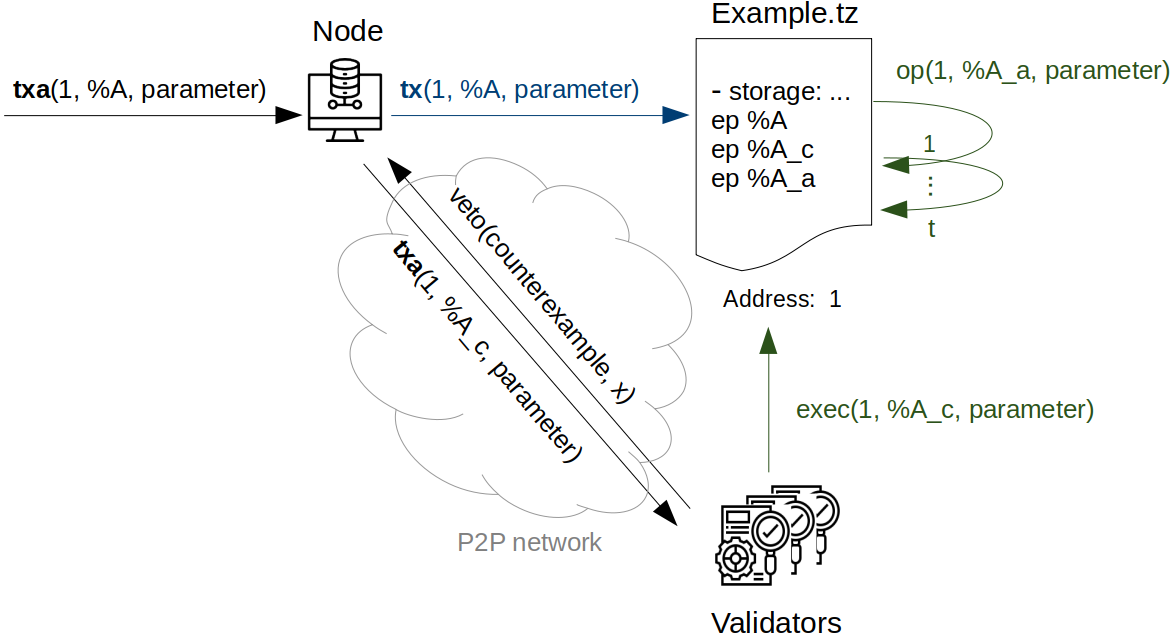
\includegraphics[width=0.7\textwidth]{figures/5-offline_tezos/interaction_monolithic_2}
	\caption{Interaction with a monolithic contract}
	\label{fig:interaction_monolithic}
\end{figure}

This orchestration scheme only works as described when using explicit entrypoint tags for the contract invocations. On the one hand, calling entrypoints implicitly by wrapping the parameter in the respective sum type constructors causes a type mismatch for the controller and assertion entrypoints. \lstref{lst:mono} shows the parameter type of the Michelson implementation corresponding to the contract given in \lstref{lst:mono_liq} --- entrypoint \texttt{A} can be invoked implicitly with parameter value \texttt{Left 4}. The respective assertion entrypoint \texttt{A\_a} expects the value as \texttt{Right (Right (Left 4))} and the controller \texttt{A\_c} as \texttt{Right (Right (Right (Left 4)))}. \\
On the other hand, the explicit tags encode the link between production, controller and assertion code --- omitting them would dissolve all references between them. Explicit entrypoints in the parameter type declaration of the contract can be enforced by the compiler. A specification of an explicit entrypoint in the contract invocation can be enforced by the \texttt{txa} operation type.
\lstinputlisting[label=lst:mono, language=Michelson, caption=Skeleton of a monolithic contract in Michelson, numbers=left]{listings/monolithic.tz}

This thesis does not go into more detail about how the described execution model for a monolithic orchestration is designed and implemented in the blockchain protocol. What needs to be considered in the protocol design is the separate execution mode, possibly a dedicated transaction type as proposed above, the derivation of a transaction which attempts to find a counterexample, the handling of assertion failures and the exclusive acceptance of either the parameter (and thus the transaction) or a counterexample.

\subsubsection{Evaluation}
The presented implementations of the monolithic approach each have strengths and weaknesses. Generally, they all share a pivotal disadvantage - they require a modification of the parent contract. This complicates the compilation process substantially and precludes the integration of assertions to contracts which have already been deployed to the blockchain. \lstref{lst:mono} shows how the parameter type and branching within the code body have to be adapted compared to the original parent contract in \lstref{lst:mono_parent}. Since the monolithic assembly result in deeper parameter and code nestings, the code becomes less readable overall.
\lstinputlisting[label=lst:mono_parent, language=Michelson, caption=Skeleton of the parent contract in Michelson, numbers=left]{listings/monolithic_parent.tz}

Another shortcoming, which applies to the implementation using separate entrypoints for controller and assertion, is the missing support of implicit entrypoint invocations. Even though the previously mentioned safety measures can prevent transactions failures, this still poses a restriction in the interaction with Smart Contracts. 

Due to the tight coupling of parent and assertion code, this approach is also inflexible. Adaptions to either the assertion or the parent contract require a complete recompilation and origination of the monolithic contract. The hybrid solution breaks some of the tight coupling, as a new version of the controller contract can be originated independently of the monolithic contract.

Besides these disadvantages, the monolithic approach has some distinct advantages. If controllers and assertions are implemented as separate entrypoints, they can be invoked independently --- this means, that the validators do not have to run the production code while checking the assertion. Conversely, the assertion code is not rerun if the parameter is valid and the transaction is broadcast to the network. This reduces the transaction cost for the user, as well as the overall footprint of the transaction on the network. If the assertion (and possibly controller) code is integrated into the parent entrypoint, this separation is not possible; however, the inseparableness the code in return avoids any bypassing of the assertion.

\subsection{Modular orchestration}\label{sec:modular}
With the modular approach, the assertion manager and each of the assertions are originated as separate contracts on the blockchain. The manager mirrors the interface of the parent contract, while each assertion each only has a single entrypoint which expects the raw parameter type. Due to the ``outsourcing'' of the assertion code, the parent contract remains pure and does not have to be modified. Similar to the hybrid solution from the last section, the manager calls the respective assertion contract $t$ times as an internal operation before calling the actual contract. In the case of empty assertions, it calls the parent contract immediately. Correspondingly, the pipeline outputs 1-$m$ contracts, where $m$ is the amount of entrypoints with an associated assertion, as depicted in \figref{fig:modular_assembly}.
\begin{figure}[h]
\centering
  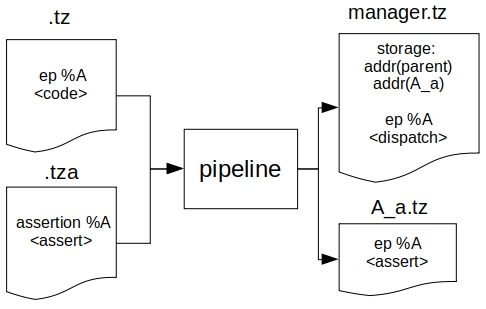
\includegraphics[width=0.6\textwidth]{figures/5-offline_tezos/pipeline_output_modular.jpg}
	\caption{Modular assembly of assertion and manager code}
	\label{fig:modular_assembly}
\end{figure}

In order to link the separate contracts to each other, the manager needs to know the addresses of the other contracts, which ultimately entails a fixed origination order. The independent assertion and parent contract(s) have been originated first, so that their addresses can be passed to the manager as initial storage values. If the storage is structured as a map from a unique identifier to an address, the entrypoints of the manager can then look up the address with its assigned identifier. The assignment of identifiers to entrypoints is hard-wired during the compilation, as is shown in the pseudocode for the manager contract in \lstref{lst:manager_modular}. The corresponding initial storage for the given contract is the mapping \texttt{{0: <addr parent>; 1: <addr A\_a>; 2: <addr B\_a}}.
\begin{lstlisting}[label=lst:manager_modular, caption=Implementation of the modular manager in pseudocode]
storage (map int address);

%A (i : int) {
	n = compute_n(i)
	Do m = 1 to n:
		call(storage.get(1), i)
	call(storage.get(0), A, i)
}

%B (j : int) {
	n = compute_n(j)
	Do m = 1 to n:
		call(storage.get(2), j)
	call(storage.get(0), B, j)
}
\end{lstlisting}

The interaction with the contracts in the modular approach is shown in \figref{fig:interaction_modular}. Even though the transactions shown in the diagram state an explicit entrypoint tag, contracts can, of course, also be called through \texttt{\%default}. In that case, the parameter passed with the internal operations to \texttt{A\_a.tz} is not equivalent, but the raw parameter value.
\begin{figure}[h]
\centering
  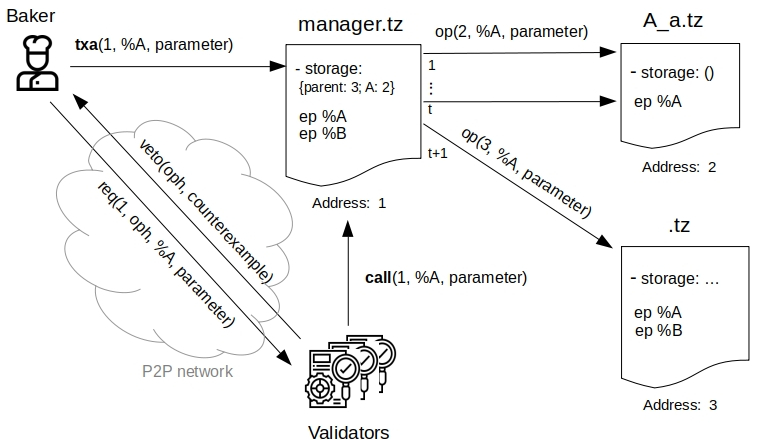
\includegraphics[width=0.9\textwidth]{figures/5-offline_tezos/interaction_modular.jpg}
	\caption{Interaction with a modular contract}
	\label{fig:interaction_modular}
\end{figure}

\subsubsection{Evaluation of the modular approach}
This approach fixes the two central problems of the monolithic approach: by mirroring the interface of the parent contract, the parameters passed to the manager contract can be forwarded directly to the parent contract, regardless of whether the default or an explicit entrypoint was called. As sum type parameters are stripped to the raw values inside the code block (ref. \lstref{lst:mono}), they can be passed to the assertion contract without further ado. Furthermore, the parent contract does not need to be modified, which leads to a much simpler compilation process and allows to extend already originated contracts with assertions. Due to its modularity, adaptions to either contract do not entail the recompilation and origination of all components. The manager is the only component with tight coupling, thus adaptions regarding the manager do not affect any other component. Adaptions to single assertions or the parent affect themselves plus the manager. In order to optimize this and break the tight coupling, one could be inclined to add a setter entrypoint to the manager (as a sort of dependency injection). This, however, would break the mirroring of the parent contract and is thus not possible without annulling one of the key strengths of the design.\\
The approach essentially has to weaknesses: on the one hand, the assertion and the parent cannot be called separately, as they are linked together by the manager. As a result, both the baker and validators execute the assertion, as well as the parent contract, which increases the cost of the contract execution. On the other hand, it exposes a security vulnerability, given that assertions can be bypassed by calling the parent contract directly with unevaluated parameters. This iteration of the design 
does not demand to close this vulnerability, hence possible solutions are not discussed in this thesis.

\section{Backend implementation}\label{sec:backend_impl}
\todo{Shorten a bit - overview already given in chpt intro}
The Tezos backend of the pipeline comprises of the three stages semantic check, type check and compilation. During the semantic check, the common AST is cast to a Tezos-specific AST type. If the assertion contains any data types or operations not supported in Michelson, the assertion contract is rejected. Since the subsequent stages are less straight forward, they are explained in more detail in the following.
\begin{figure}[h]
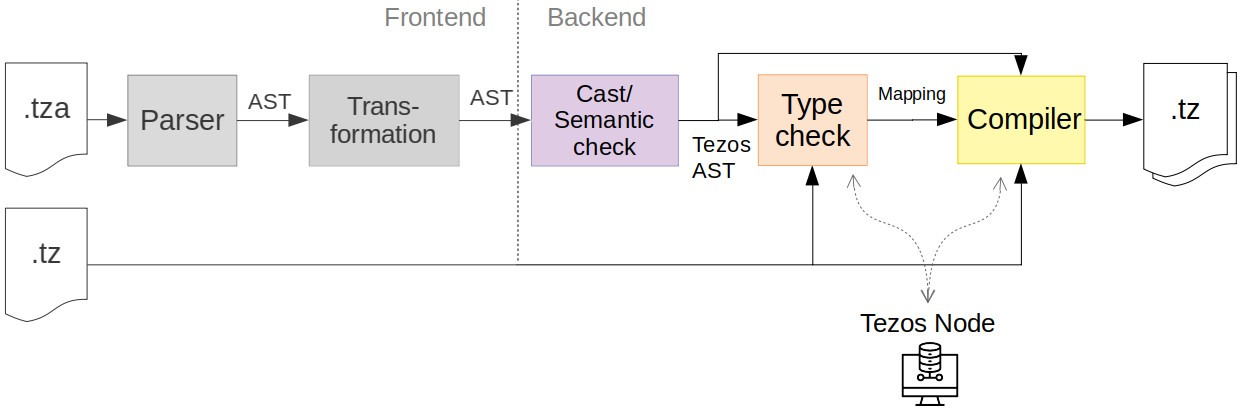
\includegraphics[width=\linewidth]{figures/5-offline_tezos/pipeline_backend}
\caption{The stages of Tezos-specific backend of the compilation pipeline}
\label{fig:pipeline_backend}
\end{figure}

\subsection{Type check}\label{sec:typecheck}
The task of the type checker is to map the assertions from the given file to the respective entrypoints of the parent contract. To this end, the parameter types have to be compared and matched against each other in order to find a correct assignment. The type checker either reads the code of the parent contract from a given file or retrieves the code from a given address on the blockchain. It must be ensured that the created mapping is injective and unambiguous, i.e., each assertion matches exactly one entrypoint and no entrypoint is covered by more than one assertion.\\
As explained in \secref{sec:tezos}, entrypoints can be selected by calling the default entrypoint and wrapping the parameter into the respective union constructors. Alternatively, they can be called explicitly using their tag and passing the parameter as raw value. The same applies for the assertions - by omitting the tag, the parameter type must be declared in respect to the default entrypoint type. If the assertion states an explicit tag, it may declare the raw parameter type. The tags do not necessarily have to be identical with the tags of the parent contract; in some cases, they may be chosen differently for documentation or for readability purposes. However, the tags can and should be used to resolve ambiguity in the mapping between assertions and entrypoints, that is if several entrypoints share the same input type. Ambiguity can also be caused by the fact that entrypoints can be sub-entrypoints of others, thus assertions overlap if a separate assertion is declared for both super- and sub-entrypoint. This is resolved by detecting overlapping assertions during the type check and rejecting assertion contracts where appropriate. \\
As an example, consider a Michelson contract with five entrypoints (including the \texttt{\%default}):
\begin{lstlisting}[numbers=none, language=Michelson]
parameter (or (int %A) (or %BC (int %B) (int %C)))
\end{lstlisting}
The following assertion contract for the given PC contains some valid and some invalid assertions:
\begin{lstlisting}[language=Assertion]
(assertion %A (i : int) ...)             (* valid *)
(assertion %D (i : int) ...)             (* invalid *)
(assertion (right (left (i : int)) ...)  (* valid *)
(assertion %BC (x : (or int int)) ...)   (* invalid *)
\end{lstlisting}
Due to its tag, the fist assertion can be assigned unambiguously to entrypoint A, whereas for the second it is not apparent whether it should be assigned to entrypoint B or C. Since the tag is omitted in the third assertion, the parameter type is given in respect to the default entrypoint and is assigned to B. The last assertion is invalid because it is overlapping with the previous assertion, which was already assigned to entrypoint B.

\subsection{Compiler}\label{sec:compiler}
The transformed and type checked assertion AST needs to be retargeted to Michelson code according to the orchestration scheme. Since the modular approach is less complex to implement and avoids having to decompile the parent code, this section describes a compiler that assembles the assertion and contract code according to \figref{fig:modular_assembly}. The target language of the compiler of the pipeline can either be Michelson directly, or another high-level language which supports Michelson as a target. \secref{sec:tezos} lists some examples of such languages. The chosen language then serves as an intermediate representation (IR) of the assertion and manager code, which is ultimately compiled to Michelson by the compiler of the language. After specifying the steps of the compilation in a general way, the compilation approaches are described and discussed in more detail in \secref{sec:direct} and \ref{sec:IR}.

\subsubsection{Compilation of the assertion contracts}
Since the assertions are independent of each other and the manager code, each of them can be compiled in isolation to a separate Michelson program. The generated code of the assertion body and the parameter type can be plugged into a template that already contains the necessary boilerplate code for a contract.
% type inference from patterns
% handling of patterns like cons

\subsubsection{Compilation of the manager contract}
Given that the manager contract mirrors the parent contract and assuming that the proposal for the storage type from \lstref{lst:manager_modular} is adopted, the type declarations can be translated directly to the target language. Algorithm \ref{alg:compile_manager} shows the outline of a simplified algorithm that builds the code body recursively. For simplicity, entrypoints that take a sum type as parameter (e.g. \texttt{(or \%AB int int)} are not considered in the algorithm. However, in the actual compiler implementation they need to be taken care of. 
\begin{algorithm}
\caption{Simplified recursive algorithm for building the manager contract}\label{alg:compile_manager}
	\begin{algorithmic}[0]
	\State global storage = \{0: <parent>\} \Comment{Stores the mapping of ids to entrypoints}
	\State global i = 1 \Comment{Counter generating unique ids}
	\Function{compile}{parent parameter type}
	\If{ty = Or(l,r)}
	\State code\_left = compile(l)
	\State code\_right = compile(r)
	\State \Return code\_left + code\_right
	\Else
	\If{assertion exists for this entrypoint}
	\State code = generate\_loop(ty, i)
	\State storage.add(i++, entrypoint tag)
	\Else
	\State code = generate\_forward(ty)
	\EndIf
	\State \Return code
	\EndIf
	\EndFunction
	\end{algorithmic}
\end{algorithm}

The function \texttt{generate\_loop} generates code that does the following:
\begin{enumerate}
\item Retrieve the assertion contract and parent contract addresses from storage
\item Calculate $t$
\item Build a list of $t$ internal operations that call the assertion contract
\item Return the list of emitted operations and the unchanged storage
\end{enumerate}
% calculate size of search space? -> need to derive a formula from range constraints
By passing the next id $i$ to the function, the access to the storage can be hard-wired into the generated code. The address of the parent contract is assumed to always be stored with the id 0. \secref{sec:prob_threshold} stated a formula for calculating $t_{total}$ with the parameters $n$, the size of the search space, and the probability threshold $c$. While $n$ can be calculated from the ranges of the random generator(s), $c$ must be given as parameter to the compiler through the CLI. After $t_{total}$ has been computed, the upper bound of the loop is calculated according to \eqref{eq:t_validator}. 
% remove -> refer to equation in previous chapter
\begin{equation}
t = \lceil t_{total} / \#validators \rceil
\end{equation}

\texttt{generate\_forward} can be generated from a simple template with the id as the only variant and only consists of  an access to the storage and the emission of an internal operation.

\subsubsection{Output}
Besides the target code for the manager and assertion contracts, the compiler should return a piece of template code for the correct storage initialization of the manager. Since this code is passed to the origination operation, it must be in Michelson regardless of the compilation target language. The placeholders or accompanying info should be descriptive enough, s.t. the user can plug in the corresponding addresses after the origination of the parent and assertion contracts. For the example manager contract given in \secref{sec:modular}, the corresponding text output could be\\
\texttt{(Elt 0 <addr parent>; Elt 1 <addr A\_a>; Elt 2 <addr B\_a>)}.

\subsubsection{Direct compilation}\label{sec:direct}
With the direct approach, the compiler generates Michelson code and hence code for a stack machine. Based on the simplicity of stack machines and the assumption that it does not need to generate optimal code, the compiler is expected to be simple \cite{cs5641}\cite{ferr_compiler}\cite{wiki:stack_machine}. As already indicate in the general part, the resulting contracts contain repeating structures and patterns for each input, which can be exploited by using template code during compilation. After compilation, the Michelson programs can be sanity-checked by type checking them using the provided Tezos libraries.

\paragraph{Assertion contracts}
\lstref{lst:contract_templ} shows a possible template for an assertion contract --- the placeholder \texttt{<?>} marks the locations where the individual code is inserted. Lines 3-5 prepare the stack, s.t. the parameter and storage are the two top elements. The lines below the placeholder for the body clean up the stack and leave it according to calling convention, i.e., the program returns an empty list of internal operations and the unit storage.
\lstinputlisting[label=lst:contract_templ, language=Michelson, caption=Template code for assertion contracts in Michelson, numbers=left]{listings/assertion_template.tz}

\paragraph{Manager contract}
The generation of the \texttt{parameter} and \texttt{storage} primitives is trivial --- the parameter type can be carried over directly from the parent contract, whereas the storage type is a constant (\texttt{(map int address)}). Based on the algorithm given previously, the code body is generated by nesting \texttt{IF\_LEFT} instructions recursively (cf. \lstref{lst:entrypoints}). The adapted algorithm is given in Algorithm \ref{alg:compile_manager_direct}.
\begin{algorithm}
\caption{Modification of algorithm \ref{alg:compile_manager} for direct compilation}\label{alg:compile_manager_direct}
	\begin{algorithmic}[0]
	\State ...
	\Function{compile}{parent parameter type}
	\If{ty = Or(l,r)} \Comment{Compile sum types to a branching}
	\State code\_left = "IF\_LEFT {" + compile(l) + "}"
	\State code\_right = "{" + compile(r) + "}"
	\State \Return code\_left + code\_right
	\EndIf
	\State ...
	\EndFunction
	\end{algorithmic}
\end{algorithm}

Owing to Michelson being a low-level language, the templates for the functions \texttt{generate\_loop} and \texttt{generate\_forward} go beyond the scope of this subsection. In order to provide an idea of how the generated code could look like, appendix \ref{apx:manager_michelson} contains two example contracts, one of which contains manager code for a non-empty and the other one for an empty assertion. The code was generated by the Liquidity compiler from two contracts written in Liquidity, as this provides a more compact and readable representation of the program logic. The corresponding source code can be found in \secref{sec:IR}.

\paragraph{Evaluation}
Compiling to Michelson directly is beneficial due of several reasons --- the pipeline stays streamlined and outputs the final contracts ready for origination. It does not introduce dependencies to external tools and their support for new protocol versions of Tezos. Besides, the new instructions only have to be added to Tezos' protocol code, whereas using external tools and languages would need to be patched as well in order to support them. \\
When it comes to verifying the compiler and integration testing of the pipeline, however, the low-level output causes more complexity than a high-level output. Due to the extend and restricted readability of non-trivial Michelson programs, their correctness is not always apparent in an instant. Tests can, on the one hand, compare the output with verified target contracts for a range of inputs, which requires a lot of Michelson code written by hand for each input. They, in turn, can also be prone to errors. \todo{remove?}On the other hand, the generated contracts can be tested as a black box using the test frameworks provided by Tezos, which use sandboxed networks to interact with contracts-under-test.


\subsubsection{Compiling to an IR}\label{sec:IR}
Instead of generating Michelson code directly, the compiler could also generate code in one of the high-level languages that provide a compiler with Michelson as a target. The output of the pipeline is then passed to this compiler in order to retrieve the final contracts. If the toolchain of the intermediate language doesn't provide a programmatic interface, the pipeline thus has to be extended with a separate step of procedure, as shown in \figref{fig:pipeline_liq}. This section demonstrates the implementation of this approach on the basis of Liquidity, hence the corresponding file extension \texttt{.liq}. \todo{provide Ligo as alternative -> could be included as package}
\begin{figure}[h]
\centering
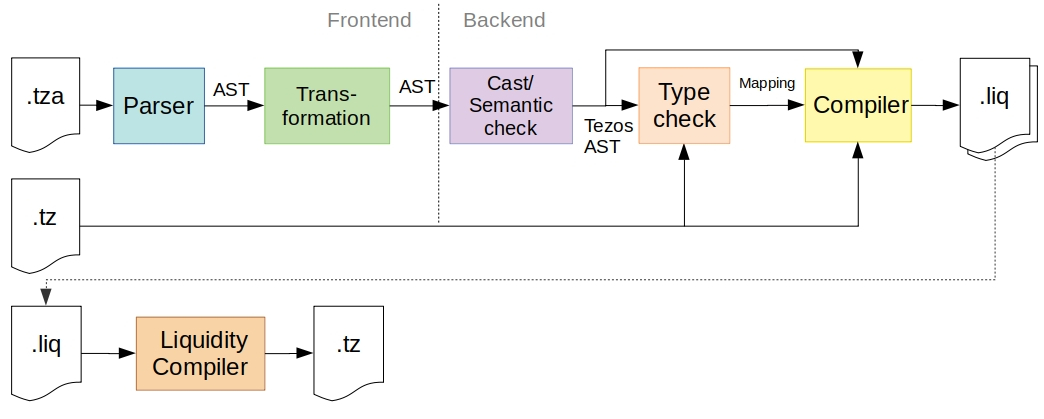
\includegraphics[width=\linewidth]{figures/5-offline_tezos/pipeline_liq}
\caption{Pipeline with IR compilation and an external toolchain}
\label{fig:pipeline_liq}
\end{figure}

\paragraph{Assertion contracts}
\lstref{lst:contract_templ_liq} shows the equivalent of the assertion contract template given in \lstref{lst:contract_templ}. Since the Liquidity compiler takes care of the handling of the stack, it basically consists only of a storage type declaration, a function signature and the ``empty'' return type.
\lstinputlisting[label=lst:contract_templ_liq, language=Michelson, caption=Template code for assertion contracts in Liquidity, numbers=left]{listings/assertion_template.liq}

\paragraph{Manager contract}
Liquidity contracts are a list of OCaml-like functions that take a parameter and a storage. Instead of declaring the contract parameter type globally and nesting the code for each entrypoint, each entrypoint thus is declared as a separate function with a local parameter type. During compilation, the contract parameter type will then be composed according to the order of functions. 
Due to Algorithm \ref{alg:compile_manager} being left recursive, the output will automatically retain the correct order of entrypoints. In fact, the only adaptions necessary are the output of the two functions \texttt{generate\_loop} and \texttt{generate\_forward}, which should not only generate the code body, but return a coherent function. The function \texttt{entrypointA} in \lstref{lst:manager_templ_liq} is an example of such a function for an empty assertion. The non-empty version of the manager code can be found in appendix \ref{apx:apx:manager_liq}. As already noted, extracting a pure template for the code exceeds the scope of this section.
\lstinputlisting[label=lst:manager_templ_liq, language=Michelson, caption=Manager code in Liquidity for an entrypoint with an empty assertion, numbers=left]{listings/manager_forward.liq}

\paragraph{Evaluation}\todo{rename?}
This approach takes advantage of the usually more sophisticated high-level language compiler; they may provide options for optimizing generated code and are already thoroughly tested \cite{liq_repo}\cite{ligo_repo}. In contract to low-level code, the output of the pipeline compiler is easier to be verified, as it can be read like, for instance, an OCaml program. Providing target contracts for integration tests can be done much more efficiently and more reliable. \\
Besides the amenities of these compilers, this approach has a crucial disadvantage of introducing an external dependency. The compiler of the respective language has to be extended with the additional Michelson instructions as well, requiring a fork of the project. Furthermore one has to rely on continuous support of new protocol versions in the root project and integrate the updates into the own codebase. All things considered, the effort for extending both Michelson and the compiler of the IR, followed by a continuous effort of version management, may outweigh the benefits of this approach.

When returning to the orchestration approach of generating a monolithic contract, using Liquidity as an IR would allow to decompile the parent contract using the decompiler of its toolchain. Since the Liquidity compiler handles the composition of the contract parameter type and the code nesting, the assertion function simply have to be appended to the parent code, which significantly decreases the compilation complexity.

\section{Cost analysis}\label{sec:cost_analysis_distributed}\todo{rename to evaluation and add some more stuff}
What remains to be evaluated is the cost of checking a formula with the proposed approach, and how they relate to the costs for a local validation which were analysed in \secref{sec:usecase_cost}. The previous analysis defined \eqref{eq:gas_transaction} to calculate the gas consumption of a transaction, including the emitted operations. For each validator, the transaction calling the manager contract emits $t+1$ internal operations, whose gas consumptions are also dependent of the input parameter. Based on the $t+1$ additional base, as well as deserialization and parsing costs of the parameter alone, it can be concluded that the total gas consumption of $n$ total distributed test runs is higher than the cost of checking $n$ values locally. \\
The differential can be measured by implementing the orchestration scheme for the two dummy contracts given in \secref{sec:usecase_cost}. Appendix \ref{apx} contains the code of all three components for each of them. In order to measure the gas consumption for a comparable amount of executions as during the initial cost analysis, the probability threshold $c$ is set to $\frac{1}{e}$, s.t. that the necessary number of total test runs is $n$. However, it needs to be pointed out, that the actual number of test runs executed can only be a multiple of the number of validators (cf. \eqref{eq:t_validator}). \figref{fig:cost_distributed} shows the reported gas consumption per validator, i.e., a $32^{th}$ of the total cost for checking an assertion for the given threshold. Due to \eqref{eq:t_validator}, the cost function approximates a step function.
\begin{figure}[t]
\centering
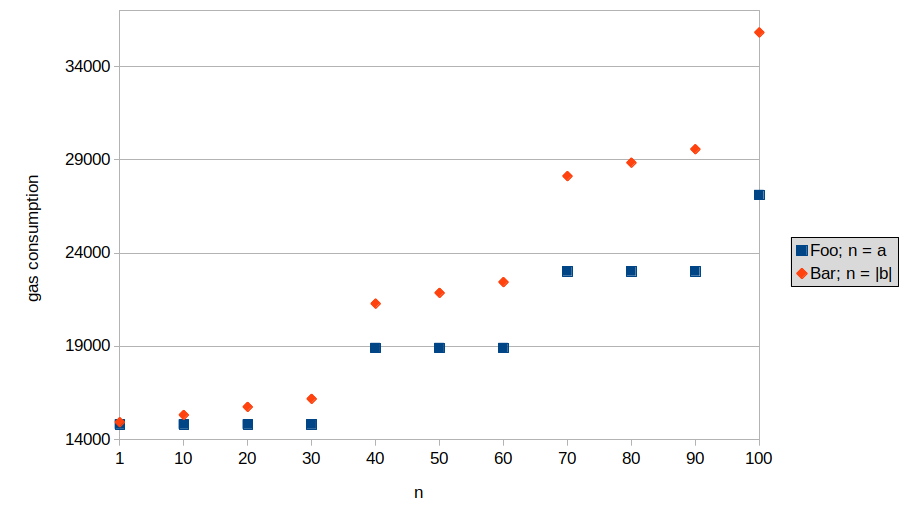
\includegraphics[width=0.9\linewidth]{figures/5-offline_tezos/cost_analysis}
\caption{Gas consumption per validator of transactions calling \texttt{Foo} and \texttt{Bar} for increasing input sizes}
\label{fig:cost_distributed}
\end{figure}
The results show that the cost incurred by a single validator checking $t$ values is already considerably higher than by checking the property locally. Moreover, the cost-performance ratio is even worse, as the confidence that the property is indeed satisfied is only around 63\% with the given parameters. In conclusion to these results, it may be worth looking into some alternative approaches. \secref{sec:alt_random} already mentions the possibility to coordinate the validators for a systematic iteration of the search space. Alternatively, the proposed orchestration could be modified, s.t. the manager and assertion code are not implemented as separate contracts, but with one single contract. Instead of $(t+1)$ internal operations, one only has to pay for one internal operation that calls the parent contract, hence avoiding the base, deserialization and parsing costs for each test run. Similar to the monolithic orchestration approach, this increases the complexity of the compilation process.\\ Another idea worth exploring is the adaption of the blockchain protocol to avoid user costs for assertion checking, similar to the regular validation of blocks \cite{tezos_docs}. Instead of being paid by the user in gas, validators could be given a reward for checking an assertion, or a particularly high one for finding a counterexample. 

\todo{Cheaper for the network if not all validators have to execute the whole local check! however, placing these costs on the users will cause them to use the local approach -> users need incentives to use it too! -> blockchain protocol could/should solve this! (e.g. use rewards instead of costs)}
\todo{Every transaction is processed at every node in the network,which limits throughput}

\section{Representing counterexamples}\label{sec:counterexample}
\todo{Adapt -> counterexample as separate contract? failwith returns address and data and validator broadcasts normal tx to this contract? is included in block and validated as any other normal tx. how to reject C(x) if A(C, x,y) is on the chain?}

There still remains an open question concerning the proposed implementation that could be answered in detail within the scope of this thesis - the representation and validation of a counterexamples. The interaction scheme in \figref{fig:interaction_modular} suggests, that validators publish an instance of a counterexample to the network if they found one. However, it has yet to be specified how the counterexample is represented and double-checked by the other validators. With the \texttt{failwith} instruction, the top element of the stack can be exposed \cite{tezos_docs}, providing a way to return an interpretable expression from the interpretation context \cite{tezos_repo}. Thus, as a first approximation, the counterexample could be represented as a tuple of assertion code and a list of randomly generated values. For instance, the counterexample for the assumption ``p is a prime'' (cf. \eqref{eq:prime}) is represented by \\
\texttt{(n >= 2 \&\& n <= sqrt(p) \&\& p\%n = 0, <random value for n>)}. \\
For validation of the counterexample, this tuple, together with the respective operation hash of the initial transaction this counterexample refers to, is published to the network. The other validators then interpret the given code with the respective value(s) and either confirm or object the counterexample. As Tezos transmits data as byte sequences, the counterexample needs to be unparsed and serialized, or deserialized and parsed respectively. If the cost for checking assertions is paid for be the user (in form of gas), then these costs have to be added to the total costs as well.\\
In order to prevent denial-of-service attacks by spamming the network with false counterexamples, the protocol should implement penalties for such cases. Details about this and possible rewards for valid counterexamples should be considered in the protocol design.


\todo{Make clear that we only engage validators on Tezos (not all nodes)}
\todo{What happens if a validator has multiple endorsing rights?}